\documentclass{article}
\usepackage{tikz}
\usepackage{amsmath}
\usepackage{algorithm}
\usepackage{algpseudocode}
\usepackage{graphicx} % Required for inserting images

\title{5800 Homework 2}
\author{Xinyan Liu}
\date{September 23rd 2024}

\begin{document}

\maketitle

\section*{2.1-1}
Using Figure 2.2 as a model, illustrate the operation of \texttt{INSERTION-SORT} on an array initially containing the sequence \{31, 41, 59, 26, 41, 58\}.

\section*{Solution}
Below are the steps demonstrating the operation of \texttt{INSERTION-SORT}:

\begin{figure}[h!]
    \centering
    % Step 1
    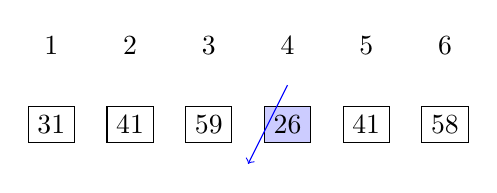
\begin{tikzpicture}
        % Array indices
        \node at (0,1) {1}; 
        \node at (1,1) {2}; 
        \node at (2,1) {3}; 
        \node at (3,1) {4}; 
        \node at (4,1) {5}; 
        \node at (5,1) {6};
        
        % Array values in rectangles
        \node[draw, rectangle] at (0,0) {31}; 
        \node[draw, rectangle] at (1,0) {41}; 
        \node[draw, rectangle] at (2,0) {59}; 
        \node[draw, rectangle, fill=blue!20] at (3,0) {26}; 
        \node[draw, rectangle] at (4,0) {41}; 
        \node[draw, rectangle] at (5,0) {58};
        
        % Arrow indicating comparison and movement
        \draw[->, blue] (3,0.5) -- (2.5,-0.5);
    \end{tikzpicture}
    \caption{(a) Initial array with key at index 4 (26)}
\end{figure}

\textbf{Explanation:} Start with the second element 41 and compare it with the first element (31). Since 41 is greater, it remains in place. Move to the third element (59). It is compared with the sorted portion {31, 41} and remains in place as it is already in the correct order. The fourth element is 26, is compared with the elements on its left. It is smaller than `59`, so `59` is moved one position to the right.

\begin{figure}[h!]
    \centering
    % Step 2
    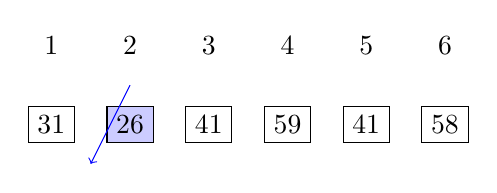
\begin{tikzpicture}
        % Array indices
        \node at (0,1) {1}; 
        \node at (1,1) {2}; 
        \node at (2,1) {3}; 
        \node at (3,1) {4}; 
        \node at (4,1) {5}; 
        \node at (5,1) {6};
        
        % Array values in rectangles
        \node[draw, rectangle] at (0,0) {31}; 
        \node[draw, rectangle, fill=blue!20] at (1,0) {26}; 
        \node[draw, rectangle] at (2,0) {41}; 
        \node[draw, rectangle] at (3,0) {59}; 
        \node[draw, rectangle] at (4,0) {41}; 
        \node[draw, rectangle] at (5,0) {58};
        
        % Arrow indicating movement
        \draw[->, blue] (1,0.5) -- (0.5,-0.5);
    \end{tikzpicture}
    \caption{(b) Inserting key 26 into the sorted portion}
\end{figure}

\text The key `26` is further compared with `41`, which is also moved to the right, until `26` is placed in its correct position before `31`.

\begin{figure}[h!]
    \centering
    % Step 3
    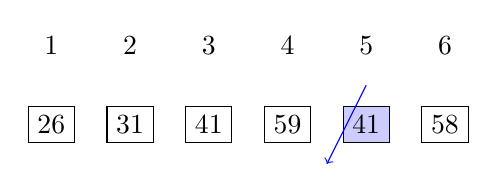
\begin{tikzpicture}
        % Array indices
        \node at (0,1) {1}; 
        \node at (1,1) {2}; 
        \node at (2,1) {3}; 
        \node at (3,1) {4}; 
        \node at (4,1) {5}; 
        \node at (5,1) {6};
        
        % Array values in rectangles
        \node[draw, rectangle] at (0,0) {26}; 
        \node[draw, rectangle] at (1,0) {31}; 
        \node[draw, rectangle] at (2,0) {41}; 
        \node[draw, rectangle] at (3,0) {59}; 
        \node[draw, rectangle, fill=blue!20] at (4,0) {41}; 
        \node[draw, rectangle] at (5,0) {58};
        
        % Arrow indicating movement
        \draw[->, blue] (4,0.5) -- (3.5,-0.5);
    \end{tikzpicture}
    \caption{(c) Inserting key 41 into the sorted portion}
\end{figure}

\text The next key `41` is already in the correct position when compared with `59`, so it is simply inserted without moving other elements.

\begin{figure}[h!]
    \centering
    % Step 4
    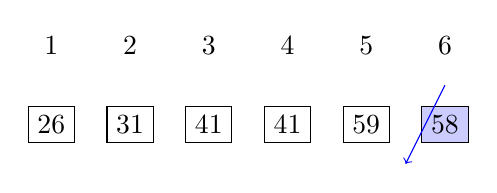
\begin{tikzpicture}
        % Array indices
        \node at (0,1) {1}; 
        \node at (1,1) {2}; 
        \node at (2,1) {3}; 
        \node at (3,1) {4}; 
        \node at (4,1) {5}; 
        \node at (5,1) {6};
        
        % Array values in rectangles
        \node[draw, rectangle] at (0,0) {26}; 
        \node[draw, rectangle] at (1,0) {31}; 
        \node[draw, rectangle] at (2,0) {41}; 
        \node[draw, rectangle] at (3,0) {41}; 
        \node[draw, rectangle] at (4,0) {59}; 
        \node[draw, rectangle, fill=blue!20] at (5,0) {58};
        
        % Arrow indicating movement
        \draw[->, blue] (5,0.5) -- (4.5,-0.5);
    \end{tikzpicture}
    \caption{(d) Inserting key 58 into the sorted portion}
\end{figure}

\text The key `58` is compared with `59`, found smaller, and inserted before it, resulting in the sorted portion up to the current element.

\begin{figure}[h!]
    \centering
    % Final sorted state
    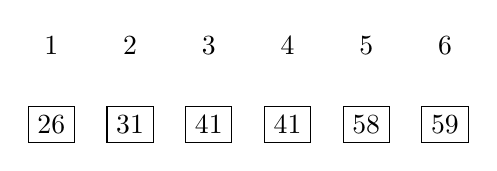
\begin{tikzpicture}
        % Array indices
        \node at (0,1) {1}; 
        \node at (1,1) {2}; 
        \node at (2,1) {3}; 
        \node at (3,1) {4}; 
        \node at (4,1) {5}; 
        \node at (5,1) {6};
        
        % Sorted array values in rectangles
        \node[draw, rectangle] at (0,0) {26}; 
        \node[draw, rectangle] at (1,0) {31}; 
        \node[draw, rectangle] at (2,0) {41}; 
        \node[draw, rectangle] at (3,0) {41}; 
        \node[draw, rectangle] at (4,0) {58}; 
        \node[draw, rectangle] at (5,0) {59};
    \end{tikzpicture}
    \caption{(e) Final sorted array}
\end{figure}

\text Follow these steps to sort the other elements in the array, the array is now completely sorted, with all elements in ascending order.

\section*{2.1-2}
Consider the procedure \texttt{SUM-ARRAY} on the facing page. It computes the sum of the numbers in the array $A[1:n]$. State a loop invariant for this procedure, and use its initialization, maintenance, and termination properties to show that the \texttt{SUM-ARRAY} procedure returns the sum of the numbers in $A[1:n]$.

\section*{Solution}

\textbf{Loop Invariant:} At the start of each iteration of the \texttt{for} loop on line 2, the variable \texttt{sum} contains the sum of the first $i-1$ elements of the array $A$, i.e., 

\[
\texttt{sum} = \sum_{j=1}^{i-1} A[j]
\]

\subsection*{Initialization}
Before the loop starts, when $i = 1$, the \texttt{sum} is initialized to 0 (line 1). This matches the invariant because there are no elements to sum in the empty subarray before the first iteration starts, so:

\[
\texttt{sum} = 0 = \sum_{j=1}^{0} A[j]
\]

Thus, the loop invariant holds at initialization.

\subsection*{Maintenance}
Proves that if the invariant holds before an iteration, and remains true after the iteration. Assume that the invariant holds at the beginning of some iteration of the loop when $i = k$ (i.e., \texttt{sum} contains the sum of the first $k-1$ elements). During this iteration, the statement \texttt{sum = sum + A[i]} adds the $k$-th element of the array $A$ to \texttt{sum}. Therefore, at the end of this iteration, \texttt{sum} contains:

\[
\texttt{sum} = \sum_{j=1}^{k-1} A[j] + A[k] = \sum_{j=1}^{k} A[j]
\]

Thus, the invariant is maintained for the next iteration.

\subsection*{Termination}
Shows that once the loop finishes, the sum is indeed the sum of the entire array. The loop terminates when $i = n + 1$, meaning the loop has iterated through all $n$ elements of $A$. \texttt{sum} contains the sum of the first $n$ elements:

\[
\texttt{sum} = \sum_{j=1}^{n} A[j]
\]

Thus, when the loop terminates, the \texttt{sum} correctly contains the sum of all the elements in the array $A[1:n]$.

Since the loop invariant holds during initialization, is maintained throughout each iteration, and holds upon termination, the \texttt{SUM-ARRAY} procedure correctly returns the sum of the numbers in the array $A[1:n]$.

\section*{2.1-5}

\text Consider the problem of adding two $n$-bit binary integers $a$ and $b$, stored in two $n$-element arrays $A[0 : n-1]$ and $B[0 : n-1]$, where each element is either $0$ or $1$. The integer $a$ can be expressed as:

\[
a = \sum_{i=0}^{n-1} A[i] \cdot 2^i
\]

Similarly, $b$ can be expressed as:

\[
b = \sum_{i=0}^{n-1} B[i] \cdot 2^i
\]

The sum $c = a + b$ of the two integers should be stored in binary form in an $(n+1)$-element array $C[0 : n]$, where:

\[
c = \sum_{i=0}^{n} C[i] \cdot 2^i
\]

Write a procedure \texttt{ADD-BINARY-INTEGERS} that takes as input arrays $A$ and $B$, along with the length $n$, and returns array $C$ holding the sum.

\section*{Solution}

\begin{algorithm}
\caption{ADD-BINARY-INTEGERS(A, B, n)}
\begin{algorithmic}[1]
\State \textbf{Input:} Arrays $A[0:n-1]$ and $B[0:n-1]$, integer $n$
\State \textbf{Output:} Array $C[0:n]$ storing the binary sum of $A$ and $B$
\State Initialize array $C[0:n]$ with all zeros
\State $carry \gets 0$
\For{$i = 0$ \textbf{to} $n-1$}
    \State $C[i] \gets A[i] + B[i] + carry$
    \If{$C[i] \geq 2$}
        \State $C[i] \gets C[i] - 2$
        \State $carry \gets 1$
    \Else
        \State $carry \gets 0$
    \EndIf
\EndFor
\State $C[n] \gets carry$
\State \textbf{return} $C$
\end{algorithmic}
\end{algorithm}

\section*{2.2-2}

\textbf Consider sorting $n$ numbers stored in array $A[1:n]$ by first finding the smallest element of $A[1:n]$ and exchanging it with the element in $A[1]$. Then find the smallest element of $A[2:n]$, and exchange it with $A[2]$. Then find the smallest element of $A[3:n]$, and exchange it with $A[3]$. Continue in this manner for the first $n - 1$ elements of $A$. Write pseudocode for this algorithm, which is known as \textit{selection sort}. What loop invariant does this algorithm maintain? Why does it need to run for only the first $n - 1$ elements, rather than for all $n$ elements? Give the worst-case running time of selection sort in $\Theta$-notation. Is the best-case running time any better?

\section*{Solution}

\subsection*{Pseudocode for Selection Sort}

\begin{algorithm}
\caption{Selection-Sort(A, n)}
\begin{algorithmic}[1]
\State \textbf{Input:} Array $A[1:n]$, integer $n$
\State \textbf{Output:} Sorted array $A$
\For{$i = 1$ \textbf{to} $n-1$}
    \State $min\_index \gets i$
    \For{$j = i+1$ \textbf{to} $n$}
        \If{$A[j] < A[min\_index]$}
            \State $min\_index \gets j$
        \EndIf
    \EndFor
    \State Swap $A[i]$ with $A[min\_index]$
\EndFor
\end{algorithmic}
\end{algorithm}

At the start of each iteration of the outer loop, the subarray $A[1:i-1]$ contains the $i-1$ smallest elements of $A$, sorted in ascending order.

\subsection*{Initialization}
Before the first iteration of the loop ($i = 1$), the subarray $A[1:0]$ is empty, which satisfies the loop invariant.

\subsection*{Maintenance}
Assume the invariant holds at the beginning of iteration $i$. At this iteration, the algorithm finds the smallest element in the subarray $A[i:n]$ and swaps it with $A[i]$. This ensures that $A[1:i]$ will be sorted and contain the $i$ smallest elements by the end of the iteration.

\subsection*{Termination}
The loop terminates when $i = n$. At this point, $A[1:n-1]$ contains the $n-1$ smallest elements, sorted in ascending order, and the last element, $A[n]$, is the largest, so the entire array is sorted.
 
The outer loop runs for the first $n-1$ elements because by the time the loop reaches the $n$-th element, it is already in the correct position. No further comparisons or swaps are necessary.


The worst-case running time of selection sort is $\Theta(n^2)$ because, in each iteration, the algorithm scans the unsorted portion of the array to find the smallest element, taking $O(n)$ time per iteration over $n-1$ iterations. The best-case running time is also $\Theta(n^2)$ because the algorithm always performs the same number of comparisons regardless of the input order.


\section*{2.2-3}

\text Consider linear search again (see Exercise 2.1-4). How many elements of the input array need to be checked on the average, assuming that the element being searched for is equally likely to be any element in the array? How about in the worst case?

Using $\Theta$-notation, give the average-case and worst-case running times of linear search. Justify your answers.

\section*{Solution}

In a linear search, the algorithm checks each element of the array sequentially until it finds the target element or reaches the end of the array. 
The expected number of checks, $E$, can be computed as:

\[
E = \frac{1 + 2 + 3 + \ldots + n}{n} = \frac{\sum_{i=1}^{n} i}{n} = \frac{\frac{n(n+1)}{2}}{n} = \frac{n+1}{2}
\]

Thus, on average, about $\frac{n+1}{2}$ elements are checked. For large $n$, this simplifies to $\Theta(n)$, which represents the average-case running time of linear search.
In the worst case, the target element is the last element of the array or not present at all. This requires checking all $n$ elements.
Therefore, the worst-case running time of linear search is \Theta(n) 

\section*{2.2-4}

\text How can you modify any sorting algorithm to have a good best-case running time?

\section*{Solution}

We can add a pre-check to determine if the input array is already sorted before running the main sorting algorithm.iterate through the array once to check if each element is less than or equal to the next element. This takes $O(n)$ time.

If the array is already sorted, we can immediately return the array as sorted without performing further operations.

If the Array is Not Sorted, then proceed to run the main sorting algorithm.

The best-case running time is $O(n)$ because the pre-check will detect an already sorted array without running the full sorting algorithm.
The worst-case running time is the same as the original sorting algorithm since the pre-check only adds a linear-time overhead.


\section*{2.3-1}

\text Using Figure 2.4 as a model, illustrate the operation of merge sort on an array initially containing the sequence $\langle 3, 41, 52, 26, 38, 57, 9, 49 \rangle$.

\section*{Solution}

\begin{figure}[h!]
    \centering
    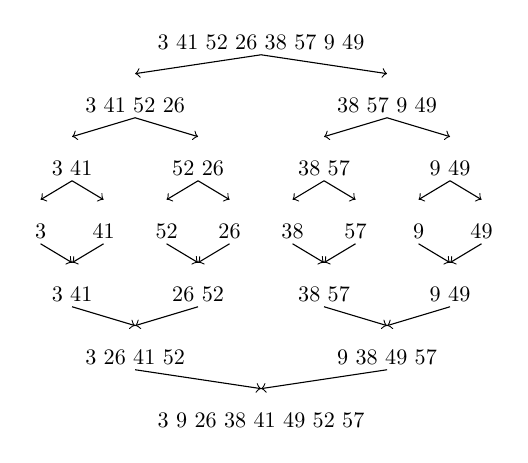
\begin{tikzpicture}[scale=0.8, every node/.style={scale=0.8}]
        % Top level - initial array
        \node at (4, 8) {3 41 52 26 38 57 9 49};
        \draw[->] (4, 7.8) -- (2, 7.5);
        \draw[->] (4, 7.8) -- (6, 7.5);
        
        % Second level - first division
        \node at (2, 7) {3 41 52 26};
        \node at (6, 7) {38 57 9 49};
        \draw[->] (2, 6.8) -- (1, 6.5);
        \draw[->] (2, 6.8) -- (3, 6.5);
        \draw[->] (6, 6.8) -- (5, 6.5);
        \draw[->] (6, 6.8) -- (7, 6.5);
        
        % Third level - second division
        \node at (1, 6) {3 41};
        \node at (3, 6) {52 26};
        \node at (5, 6) {38 57};
        \node at (7, 6) {9 49};
        \draw[->] (1, 5.8) -- (0.5, 5.5);
        \draw[->] (1, 5.8) -- (1.5, 5.5);
        \draw[->] (3, 5.8) -- (2.5, 5.5);
        \draw[->] (3, 5.8) -- (3.5, 5.5);
        \draw[->] (5, 5.8) -- (4.5, 5.5);
        \draw[->] (5, 5.8) -- (5.5, 5.5);
        \draw[->] (7, 5.8) -- (6.5, 5.5);
        \draw[->] (7, 5.8) -- (7.5, 5.5);
        
        % Fourth level - third division
        \node at (0.5, 5) {3};
        \node at (1.5, 5) {41};
        \node at (2.5, 5) {52};
        \node at (3.5, 5) {26};
        \node at (4.5, 5) {38};
        \node at (5.5, 5) {57};
        \node at (6.5, 5) {9};
        \node at (7.5, 5) {49};
        \draw[->] (0.5, 4.8) -- (1, 4.5);
        \draw[->] (1.5, 4.8) -- (1, 4.5);
        \draw[->] (2.5, 4.8) -- (3, 4.5);
        \draw[->] (3.5, 4.8) -- (3, 4.5);
        \draw[->] (4.5, 4.8) -- (5, 4.5);
        \draw[->] (5.5, 4.8) -- (5, 4.5);
        \draw[->] (6.5, 4.8) -- (7, 4.5);
        \draw[->] (7.5, 4.8) -- (7, 4.5);
        
        % Fifth level - first merge
        \node at (1, 4) {3 41};
        \node at (3, 4) {26 52};
        \node at (5, 4) {38 57};
        \node at (7, 4) {9 49};
        \draw[->] (1, 3.8) -- (2, 3.5);
        \draw[->] (3, 3.8) -- (2, 3.5);
        \draw[->] (5, 3.8) -- (6, 3.5);
        \draw[->] (7, 3.8) -- (6, 3.5);
        
        % Sixth level - second merge
        \node at (2, 3) {3 26 41 52};
        \node at (6, 3) {9 38 49 57};
        \draw[->] (2, 2.8) -- (4, 2.5);
        \draw[->] (6, 2.8) -- (4, 2.5);
        
        % Final merge
        \node at (4, 2) {3 9 26 38 41 49 52 57};
    \end{tikzpicture}
    \caption{The operation of merge sort on the array \{3, 41, 52, 26, 38, 57, 9, 49\}.}
\end{figure}


1. The array is recursively divided into smaller subarrays until each subarray contains a single element.
2. The subarrays are then merged step-by-step in sorted order until the entire array is sorted.

\section*{2.3-3}

\textbf State a loop invariant for the \texttt{while} loop of lines 12–18 of the \texttt{MERGE} procedure. Show how to use it, along with the \texttt{while} loops of lines 20–23 and 24–27, to prove that the \texttt{MERGE} procedure is correct.

\section*{Solution}

\subsection*{Loop Invariant for Lines 12–18}

\textbf{Invariant:} At the start of each iteration of the \texttt{while} loop (lines 12–18), the subarray $A[p:k-1]$ contains the smallest elements of the merged subarrays $L$ and $R$, sorted in non-decreasing order. Additionally, all elements in $L[i:]$ and $R[j:]$ are yet to be merged.

\begin{itemize}
    \item \textbf{Initialization:} Before the first iteration, $k = p$, and no elements have been merged, so $A[p:k-1]$ is empty, which trivially satisfies the invariant.
    \item \textbf{Maintenance:} During each iteration, either $L[i]$ or $R[j]$ (the smaller of the two) is appended to $A[k]$, incrementing $k$. The invariant holds since $A[p:k]$ remains sorted.
    \item \textbf{Termination:} The loop terminates when either $i = n_L$ or $j = n_R$, meaning one of the subarrays has been completely merged into $A[p:r]$.
\end{itemize}

\subsection*{Loops in Lines 20–23 and 24–27}

These loops append the remaining elements from $L$ or $R$ (whichever has elements left) to $A$, preserving sorted order.

\section*{2.3-8}

\textbf Describe an algorithm that, given a set $S$ of $n$ integers and another integer $x$, determines whether $S$ contains two elements that sum to exactly $x$. Your algorithm should take $\Theta(n \log n)$ time in the worst case.

\section*{Solution}

\textbf{Algorithm:}
\begin{enumerate}
    \item Sort the array $S$ in $\Theta(n \log n)$ time.
    \item Initialize two pointers: one at the beginning ($i = 1$) and one at the end ($j = n$) of the sorted array.
    \item While $i < j$:
    \begin{itemize}
        \item Compute the sum $s = S[i] + S[j]$.
        \item If $s = x$, return \texttt{true}.
        \item If $s < x$, increment $i$ to increase the sum.
        \item If $s > x$, decrement $j$ to decrease the sum.
    \end{itemize}
    \item If no such pair is found, return \texttt{false}.
\end{enumerate}

\textbf{Time Complexity:} Sorting takes $\Theta(n \log n)$, and the two-pointer scan runs in $O(n)$, making the overall time complexity $\Theta(n \log n)$.

\section*{Problem 2-3: Correctness of Horner's Rule}

The function \texttt{horner} evaluates a polynomial given its coefficients and a value $x$. It processes the coefficients from the highest power to the lowest using the recurrence:

\[
P(x) = a_0 + x(a_1 + x(a_2 + \ldots + x(a_{n-1} + x a_n) \ldots))
\]

\subsection*{Binary to Decimal Conversion}

The \texttt{binaryToDecimal} function uses Horner’s rule to convert a binary number (represented as a vector of bits) into its decimal form by treating the binary digits as coefficients and using $2$ as the base.

You are given the coefficients $a_0, a_1, a_2, \ldots, a_n$ of a polynomial

\[
P(x) = \sum_{k=0}^{n} a_k x^k = a_0 + a_1 x + a_2 x^2 + \cdots + a_{n-1} x^{n-1} + a_n x^n,
\]

and you want to evaluate this polynomial for a given value of $x$. \textit{Horner's rule} says to evaluate the polynomial according to this parenthesization:

\[
P(x) = a_0 + x \left( a_1 + x \left( a_2 + \cdots + x \left(a_{n-1} + x a_n \cdots \right) \right) \right).
\]

The procedure \texttt{HORNER} implements Horner's rule to evaluate $P(x)$, given the coefficients $a_0, a_1, a_2, \ldots, a_n$ in an array $A[0:n]$ and the value of $x$.

\begin{verbatim}
HORNER(A, n, x)
1    p = 0
2    for i = n downto 0
3        p = A[i] + x * p
4    return p
\end{verbatim}

\begin{enumerate}
    \item[a.] In terms of $\Theta$-notation, what is the running time of this procedure?
    
    \item[b.] Write pseudocode to implement the naive polynomial-evaluation algorithm that computes each term of the polynomial from scratch. What is the running time of this algorithm? How does it compare with \texttt{HORNER}?
    
    \item[c.] Consider the following loop invariant for the procedure \texttt{HORNER}:
    
    At the start of each iteration of the \texttt{for} loop of lines 2–3,
    
    \[
    p = \sum_{k=0}^{n-(i+1)} A[k + i + 1] \cdot x^k.
    \]
    
    Interpret a summation with no terms as equaling 0. Following the structure of the loop-invariant proof presented in this chapter, use this loop invariant to show that, at termination,
    
    \[
    p = \sum_{k=0}^{n} A[k] \cdot x^k.
    \]
\end{enumerate}

\section*{Solutions}

\begin{enumerate}
    \item[a.] The running time of the procedure \texttt{HORNER} in terms of $\Theta$-notation is:
    
    \[
    \Theta(n)
    \]
    
    \item[b.] Pseudocode for the naive polynomial evaluation algorithm:
    
    \begin{verbatim}
    NAIVE_POLYNOMIAL(A, n, x)
        p = 0
        for i = 0 to n
            term = A[i]
            for j = 1 to i
                term = term * x
            p = p + term
        return p
    \end{verbatim}
    
    The running time of this algorithm is:
    
    \[
    \Theta(n^2)
    \]
    
    Comparison: The naive approach has a time complexity of $\Theta(n^2)$ because it computes each power of $x$ from scratch for each term, whereas \texttt{HORNER} has a time complexity of $\Theta(n)$, making \texttt{HORNER} significantly more efficient.
    
    \item[c.] The loop invariant at the start of each iteration of the \texttt{for} loop of lines 2–3 is:
    
    \[
    p = \sum_{k=0}^{n-(i+1)} A[k + i + 1] \cdot x^k.
    \]
    
    At termination, $i = -1$, and the invariant shows that $p$ correctly evaluates the polynomial:
    
    \[
    p = \sum_{k=0}^{n} A[k] \cdot x^k.
    \]
    
    This confirms that the loop invariant holds, and the final value of $p$ is the correct evaluation of the polynomial.

C++ implementations Please see attached Horner_Rule.cpp


\end{enumerate}

\end{document}